\chapter{Session}

\section{用語}

\begin{dfn}
  \textbf{Context Manager}
\end{dfn}

with文に渡されるオブジェクトの総称を context managerと言います。
context managerの中では、\_\_enter\_\_と\_\_exit\_\_というそれぞれ前処理と後処理を定義した特殊メソッドが実装されています。
sessionにおいては、SQLを発行した後にそれが必ずcommitされ、さらにデータベースへの接続を必ず閉じるためにこのcontext managerが利用されます。


\section{いつ使う?}
\begin{itemize}
  \item {ORMを使ってDBを操作するときに必ず使います。}
\end{itemize}



\section {Sessionの役割}

\subsection{インターフェースの提供}
\label{session.interface}
Engineの役割はPoolとDialectを操作してDBAPIからDBMSを操作することでした。
対してSessionの役割は、\textbf{Engineを操作するためのインターフェースを提供すること}です。
図\ref{session}を見てください。一般的に、engineはプロセス内で1つだけ生成されます。
engineに対して、sessionはクエリが発行されるなどのDBに対する処理を行うたびに生成され、その度に破棄されます。
以下にsessionが生成されてから破棄されるまでのライフサイクルを説明していきます。
\\

\begin{figure}[H]
\begin{center}
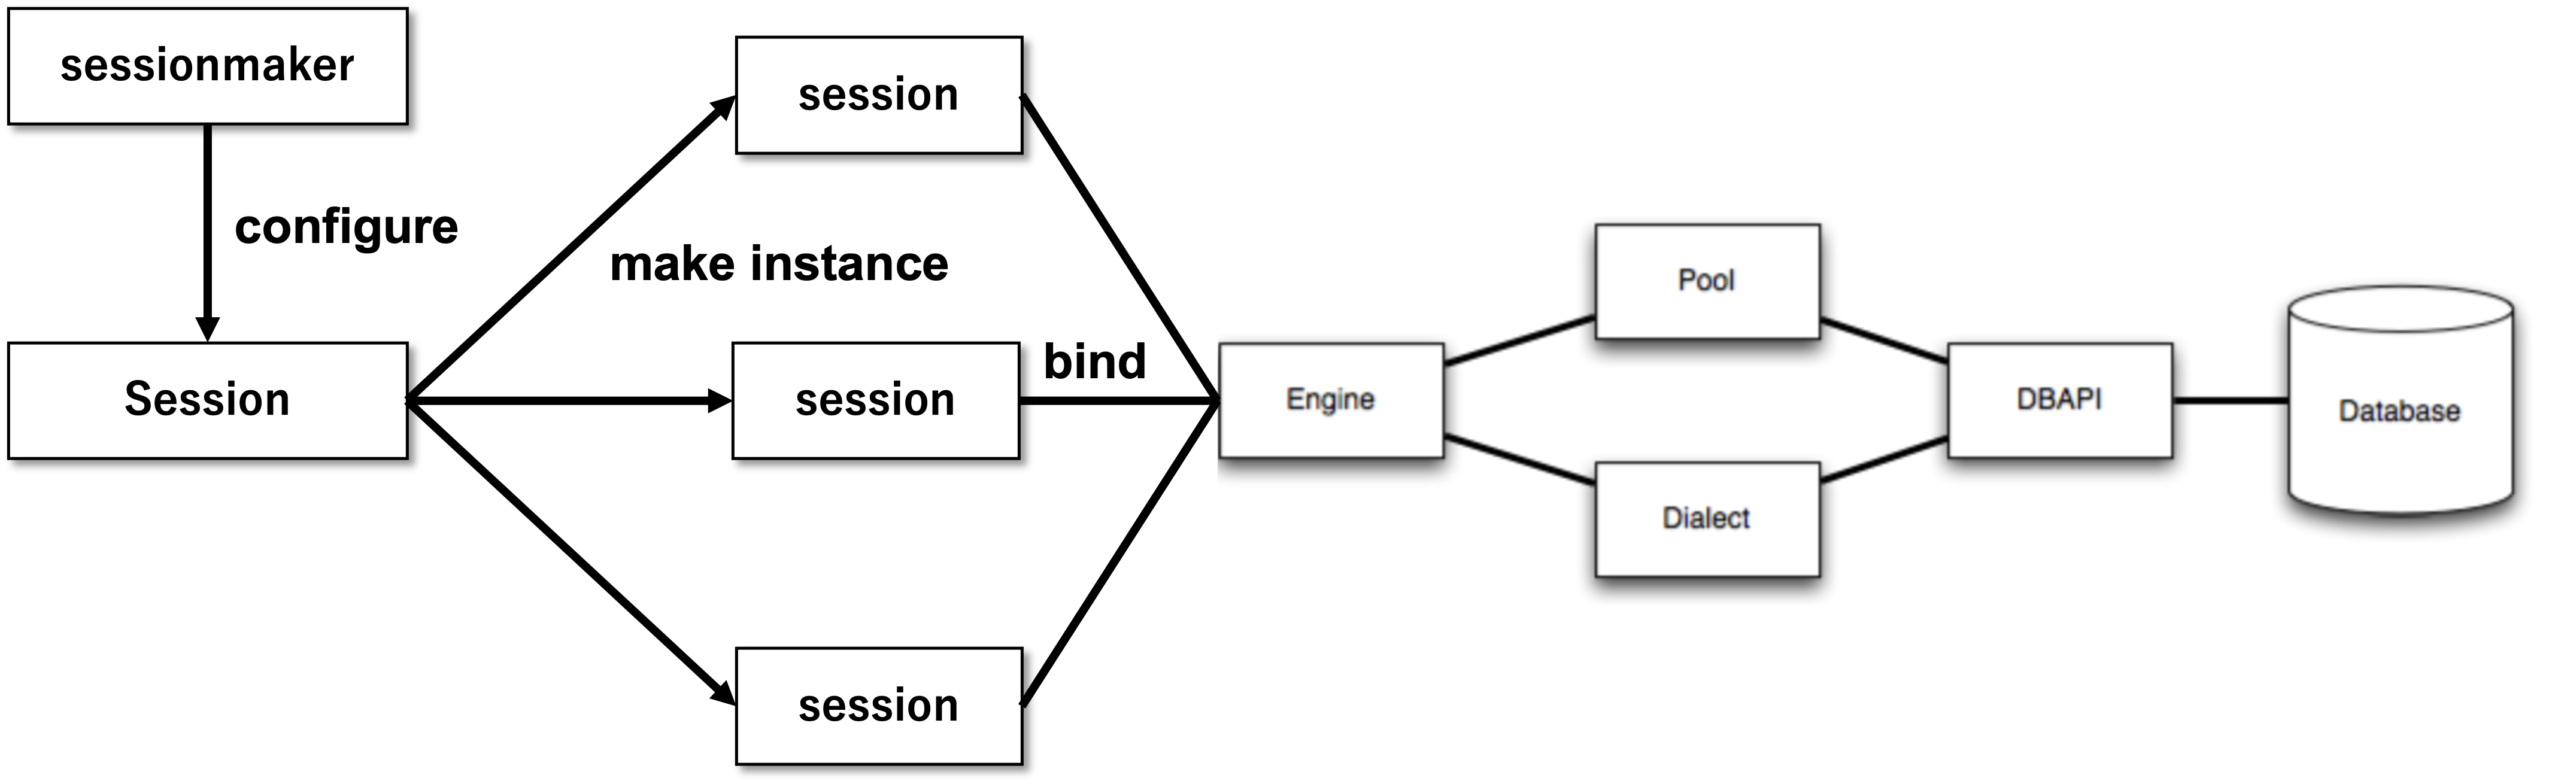
\includegraphics[width=14cm]{session/session.png}
\caption{sessionの役割}
\label{session}
\end{center}
\end{figure}

\subsection{コンテクストマネージャ}
Sessionはコンテクストマネージャとしての役割を持っています。
コンテクストマネージャは、特定の処理の最後に必ず行う \_\_exit\_\_を自動的に行ってくれるのでした。
Sessionクラスをインスタンス化したsessionが生成され、処理が終了したのちに、\textbf{session.close()}が必ず呼び出され、DBへの処理の間に保持していたORMオブジェクトやconnectionオブジェクトを全て破棄します。

\begin{lstlisting}[caption={コンテクストマネージャ}]
  with Session(engine) as session:
    session.add(some_object)
    session.add(some_other_object)
    session.commit()
\end{lstlisting}


\section{sessionmaker}

\subsection{どこで呼び出すべきか?}
チュートリアルや他の解説記事では1つの.pyファイルの中でsessionの生成を行っていますが、実際にはモジュールごとに分割して管理することが多いはずです。
その際に、sessionmakerはグローバルスコープで1回のみ呼ぶようにして、他のモジュールはimportでSessionを呼ぶようにしてください。
